%%% Preamble
\documentclass[11pt]{article}

\usepackage[paper=A4,pagesize]{typearea}
\usepackage[utf8]{inputenc}
\usepackage[T1]{fontenc}
\usepackage[a4paper,pdftex]{geometry}	% Use A4 paper margins
\usepackage[french]{babel}
\usepackage{xcolor} % Required for specifying custom colors
\usepackage{fix-cm} % Allows increasing the font size of specific fonts beyond LaTeX default specifications
\usepackage{hyperref}
\usepackage{todonotes}
\usepackage{wrapfig}
\usepackage{pdfpages}
\usepackage{afterpage}
\usepackage{csvsimple}
\usepackage{float}
\restylefloat{table,figure}

%%% Begin document
\begin{document}
\includepdf[pages={1}]{title.pdf}

% Liste des TODOs
%\listoftodos[Modifications du rapport]
%\newpage

\tableofcontents

\listoffigures

\listoftables

\newpage

\part{Livrables}

\section{Déroulement et répartition des tâches}

Durant ce projet, nous devions implémenter un analyseur et interpréteur du langage de programmation \textit{lutin}. Pour ce faire, nous avons suivi les étapes de travail proposées dans le sujet en attribuant des membres sur chacune d'elles, permettant ainsi de les paralléliser. \\

Dans un premier temps, tout le monde a réfléchi à la grammaire du langage, puis nous avons choisi celle qui était la plus simple et la plus compréhensible par l'équipe. Nous l'avons ensuite transformé en grammaire LR, visible dans la section \ref{sec:grammaire}. \\

Nous avons ensuite avancé en parallèle sur les tâches ci-dessous avant de nous consacrer à l'implémentation :
\begin{itemize}
	\item Construction de l'automate LR correspondant (voir section \ref{sec:automate}) puis réalisation de la table des transitions (voir section \ref{sec:transitions}) (par Jonathan, Nicolas et Romain)
	\item Conception de la structure de données sous forme de diagramme UML \ref{sec:structure} (par Antoine, Pierre et Baptiste)
	\item Identification des expressions régulières (par Benoît) \\
\end{itemize}

Enfin, nous avons procédé à l'implémentation de cet analyseur et interpréteur de la manière suivante :
\begin{itemize}
	\item Implémentation de l'analyseur lexical (par Jonathan)
	\item Implémentation de l'automate LR (par Antoine et Benoît)
	\item Réalisation de l'outil en ligne de commande (par Baptiste)
	\item Vérification statique du programme (par Pierre)
	\item Implémentation de toutes les classes symboles (par Nicolas et Romain)
	\item Conception de la partie optimisation et son implémentation (par Pierre et Baptiste)
	\item Conception et réalisation de la partie affichage du programme en mémoire (par Jonathan)
	\item Mise en place des gestions d'erreurs lexicales et syntaxiques et récupération (par Antoine, Benoît et Pierre)
	\item Implémentation des tests (par toute l'équipe)\\
\end{itemize}

À titre indicatif, pour terminer ce projet nous avons passé, en dehors des séances, en moyenne 8 heures chacun.

\newpage

\section{Grammaire du langage lutin}
\label{sec:grammaire}

Vous trouverez dans le tableau ci-dessous (cf. tableau \ref{tab:grammaire}), l'ensemble des règles de notre grammaire pour le langage lutin, numérotées pour faciliter la compréhension de la table de transition (voir section \ref{sec:transitions}). Le symbole $\epsilon$ représente l’élément vide.

\begin{table}[h]
	\centering
	\begin{tabular}{|c|l c l|}
		\hline
		Numéro & \multicolumn{3}{c|}{Règle} \\
		\hline
		1 & P & $\rightarrow$ & D I \\
		2 & D & $\rightarrow$ & D D’ \\
		3 & D & $\rightarrow$ & $\epsilon$ \\
		4 & D’ & $\rightarrow$ & var V ; \\
		5 & D’ & $\rightarrow$ & const C ; \\
		6 & V & $\rightarrow$ & V , id \\
		7 & V & $\rightarrow$ & id \\
		8 & C & $\rightarrow$ & C , id = val \\
		9 & C & $\rightarrow$ & id = val \\
		10 & I & $\rightarrow$ & I I’ \\
		11 & I & $\rightarrow$ & I’ \\
		12 & I’ & $\rightarrow$ & lire id ; \\
		13 & I’ & $\rightarrow$ & ecrire E ; \\
		14 & I’ & $\rightarrow$ & id := E ; \\
		15 & E & $\rightarrow$ & E + E \\
		16 & E & $\rightarrow$ & E * E \\
		17 & E & $\rightarrow$ & E - E \\
		18 & E & $\rightarrow$ & E / E \\
		19 & E & $\rightarrow$ & ( E ) \\
		20 & E & $\rightarrow$ & id \\
		21 & E & $\rightarrow$ & val \\
		\hline
	\end{tabular}
	\caption{Grammaire du langage lutin}
	\label{tab:grammaire}
\end{table}

%% Section : Automate LR
\afterpage{
	\clearpage
	\KOMAoptions{paper=A3,pagesize,paper=landscape,DIV=20}
	\recalctypearea
	\section{Automate LR}
	\label{sec:automate}

	Vous trouverez ci-dessous (cf. figure \ref{fig:automate}) le schéma décrivant l'automate LR de notre grammaire permettant d'identifier les différents états et transitions avant l'implémentation.
	
	\begin{figure}[H]
		\centerline{
			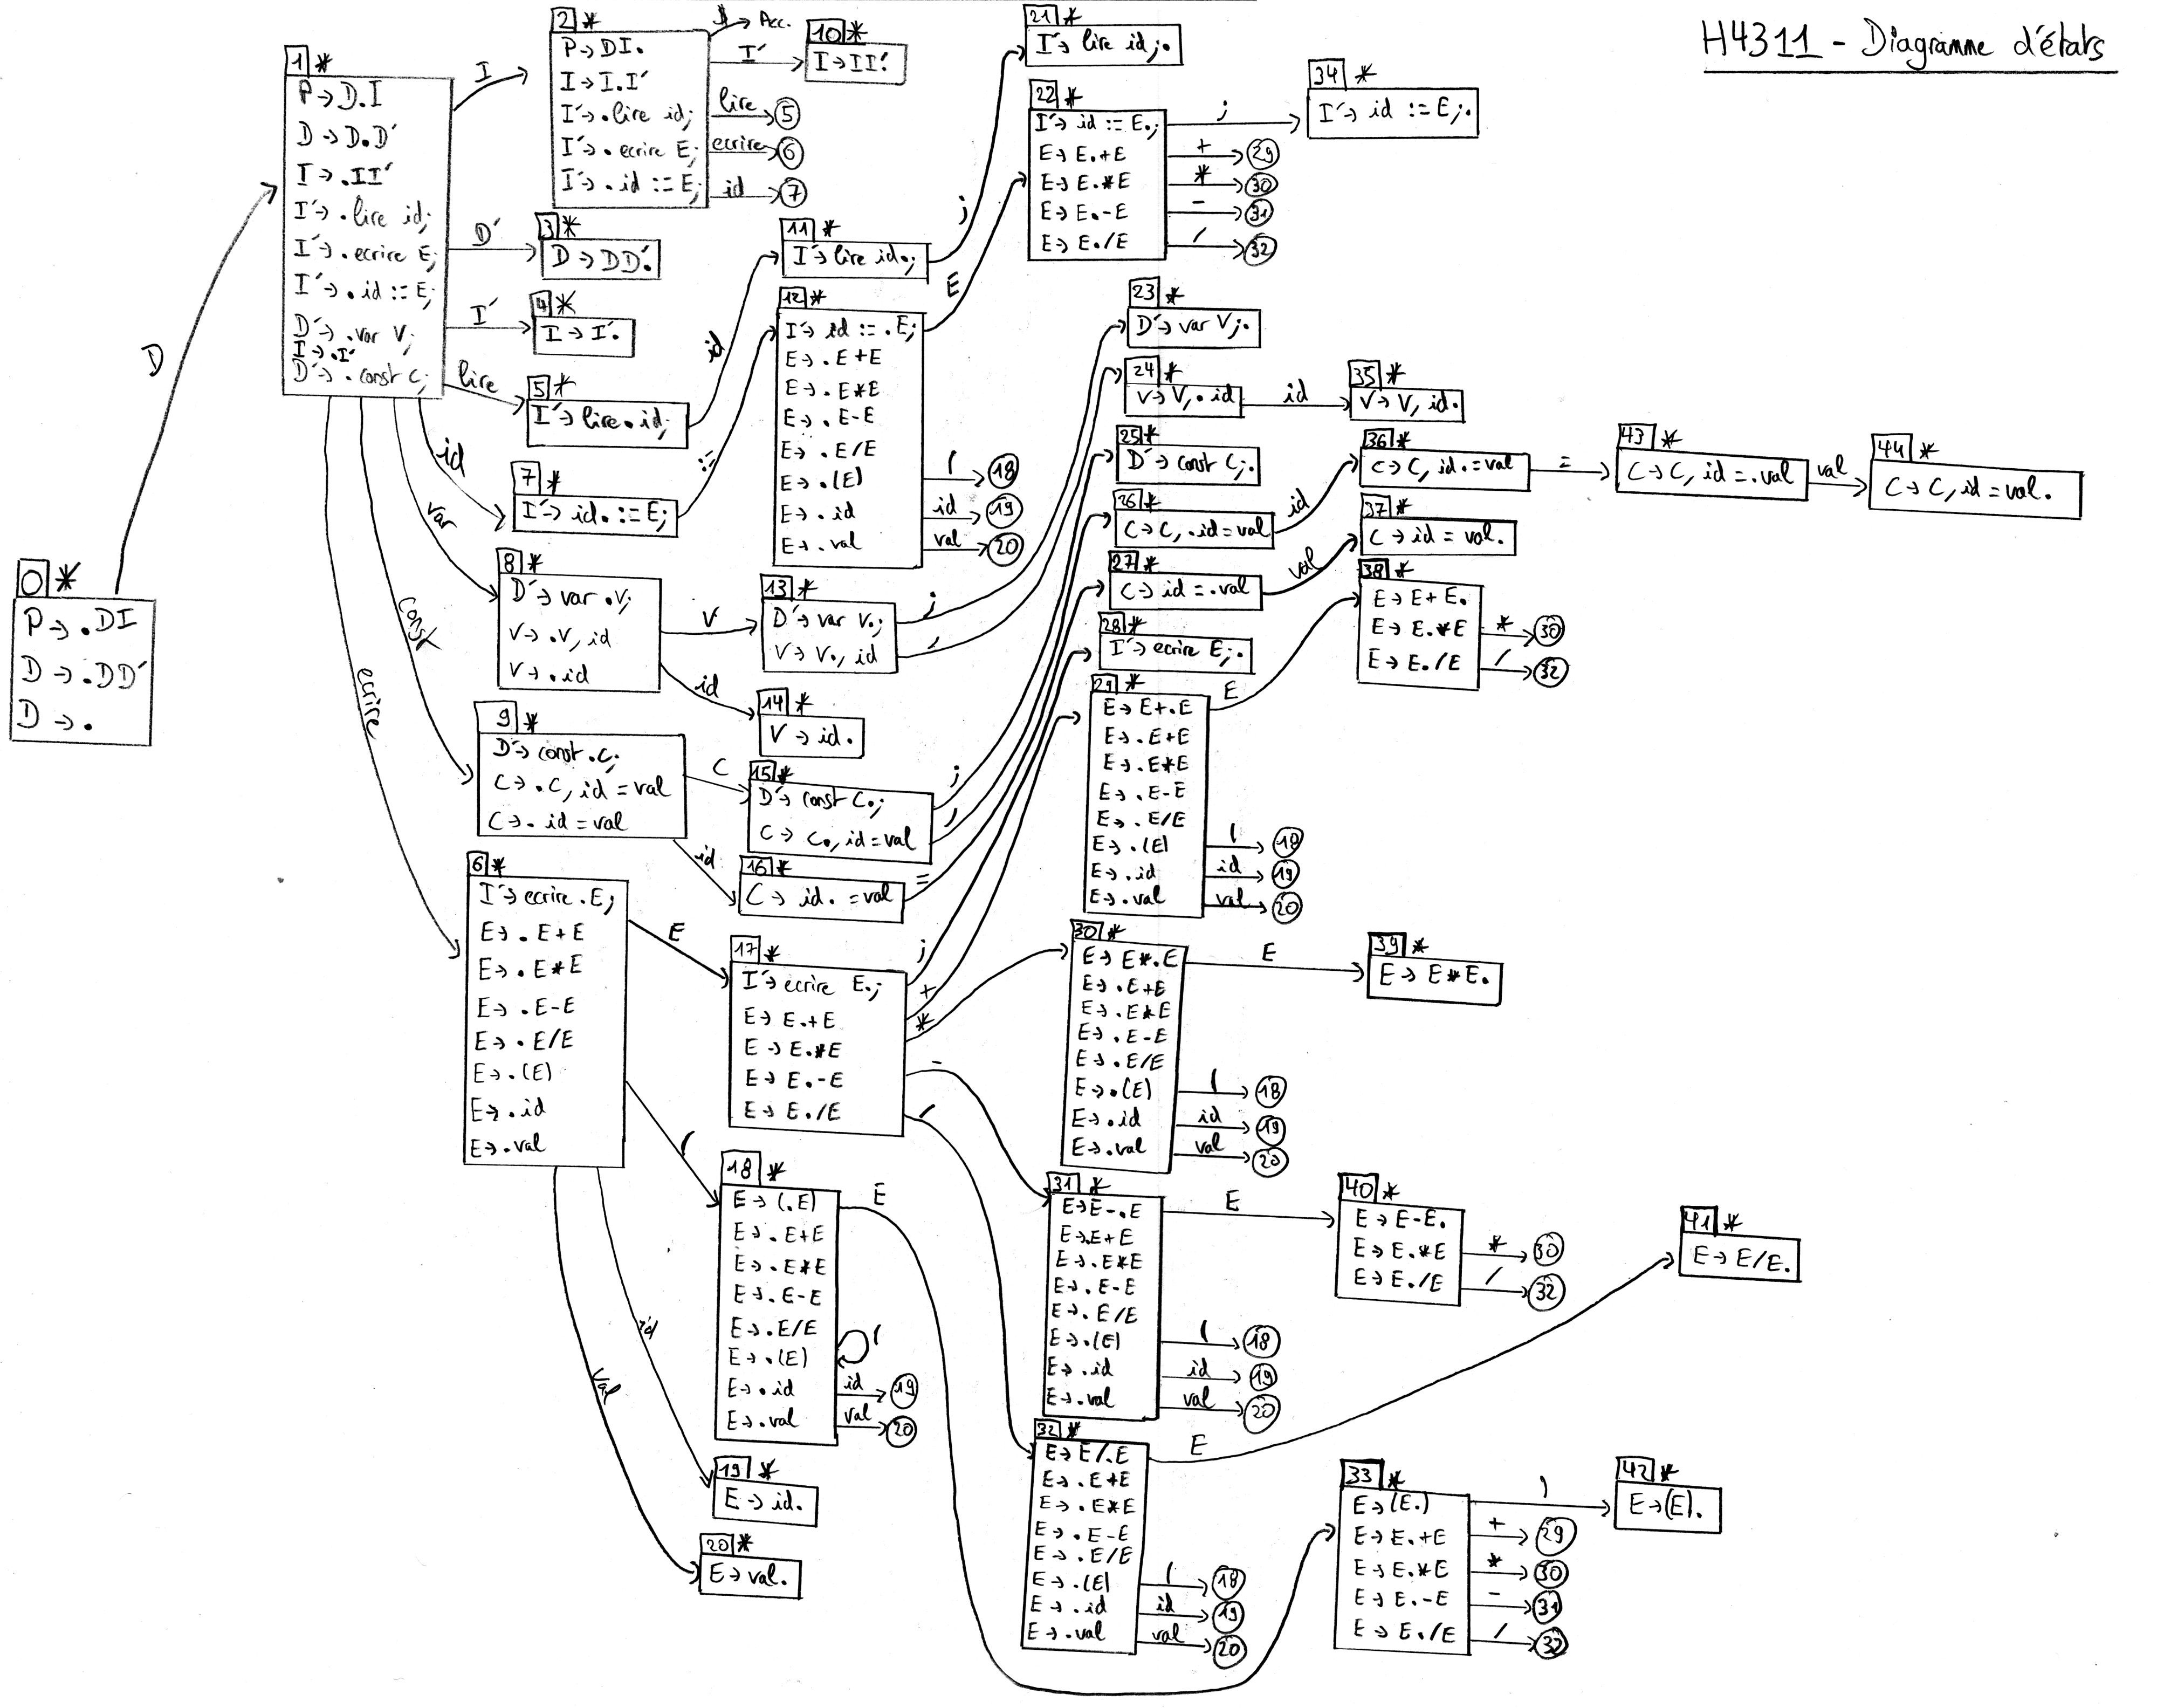
\includegraphics[height=0.85\textheight,width=1.0\textwidth,keepaspectratio]{figures/automate-LR-lutin.jpg}
		}
		\caption{Automate LR par rapport à la grammaire du langage lutin}
		\label{fig:automate}
	\end{figure}

	\clearpage
	\KOMAoptions{paper=A4,pagesize}
	\recalctypearea
}

%% Section : Table des transitions LR
\afterpage{
	\clearpage
	\KOMAoptions{paper=A3,pagesize,paper=landscape,DIV=20}
	\recalctypearea
	\section{Table des transitions LR}
	\label{sec:transitions}

	Avant d'implémenter l'ensemble des états, nous avons réalisé une table référençant toutes les transitions possibles d'un état à un autre en fonction des symboles analysés. Voici cette table de transition LR (cf tableau \ref{tab:transitions}).
	
	\begin{table}[H]
		\centering
		\csvautotabular[respect dollar=true]{data/table-analyse-automate-lr.csv}
		\label{tab:transitions}
		\caption{Table des transitions LR}
	\end{table}

	\clearpage
	\KOMAoptions{paper=A4,pagesize}
	\recalctypearea
}

%% Section : Structures de données
\afterpage{
	\clearpage
	\KOMAoptions{paper=A3,pagesize,paper=landscape,DIV=20}
	\recalctypearea
	\section{Structures de données}
	\label{sec:structure}
	
	Afin de décrire au mieux la structure employée dans ce projet, vous trouverez ci-dessous le diagramme de classes simplifié dans le standard UML (cf. figure \ref{fig:structure}). En effet, afin de le rendre plus compréhensible, seules les classes les plus importantes sont visibles, les classes de type exception étant également regroupées dans un package. Vous trouverez en annexe (cf. figure \ref{fig:full-structure}) le diagramme de classes complet du programme.

	\begin{figure}[H]
		\centerline{
			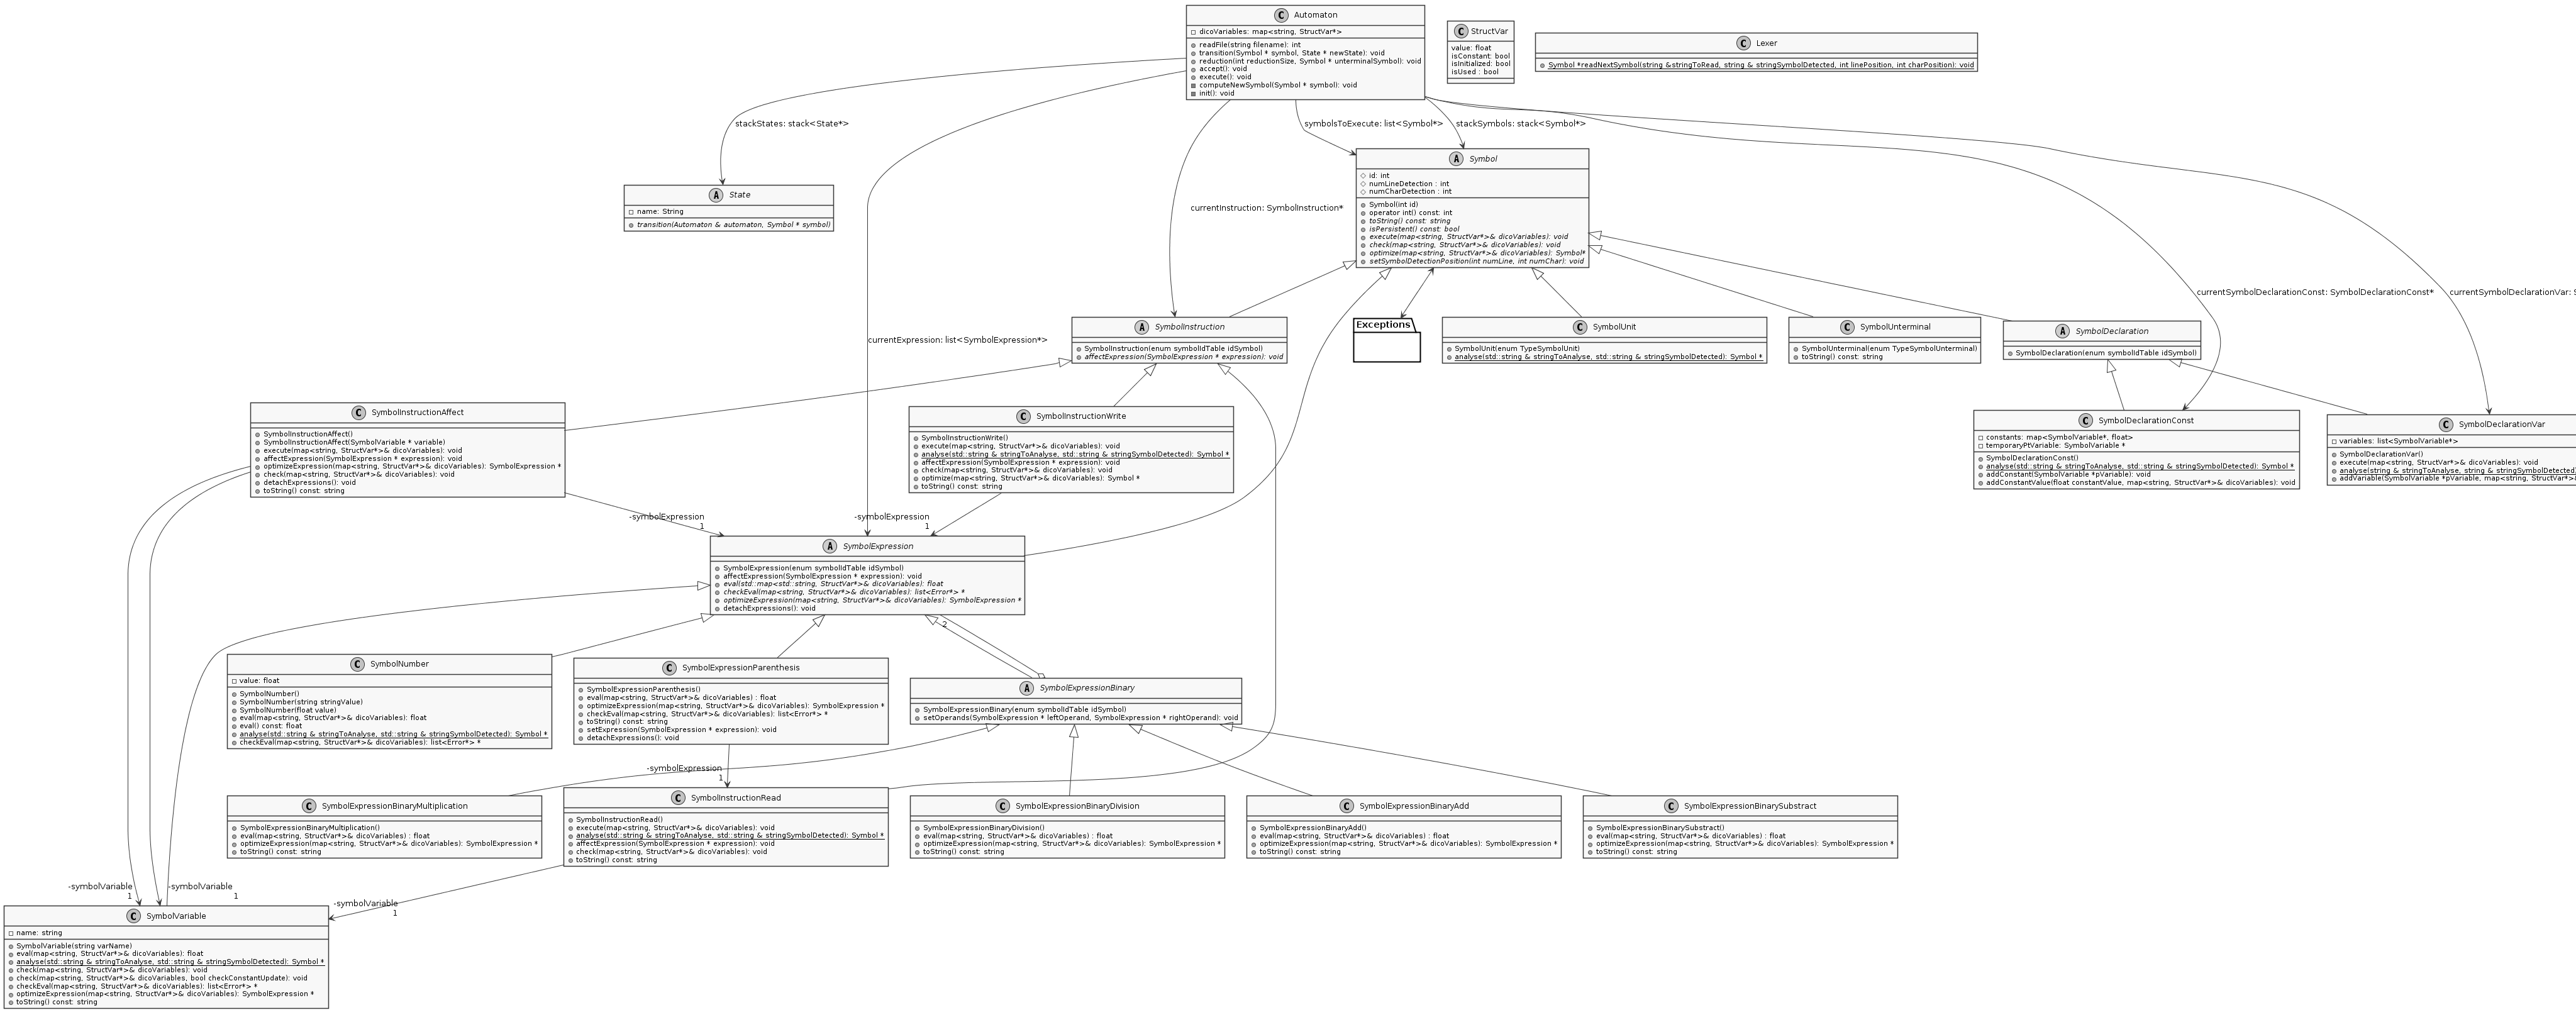
\includegraphics[width=1.15\textwidth,keepaspectratio]{../diagrams-simplified/class/lutin-compiler-class-diagram-simplified-uml.png}
		}
		\label{fig:structure}
		\caption{Diagramme de classes des structures de données}
	\end{figure}

	\clearpage
	\KOMAoptions{paper=A4,pagesize}
	\recalctypearea
}

% Annexes
\afterpage{
	\clearpage
	\KOMAoptions{paper=A3,pagesize,paper=landscape,DIV=20}
	\recalctypearea
	
	\part{Annexes}
	
	\section{Gestion des erreurs}
	\label{sec:erreurs}
	
	\subsection{Listes des erreurs traitées}
	\label{subsec:erreur-liste}	
	
	\begin{table}[h]
		\centering
		\begin{tabular}{|c|c|c|}
			\hline
			\textbf{Erreur} & \textbf{Type} & \textbf{Code de retour} \\
			\hline
			Problème dans les arguments & Arguments & 1 \\
			\hline
			Impossible d'ouvrir le fichier & I/O & 2 \\
			\hline
			Variable déjà déclarée & Semantique & 3 \\
			\hline
			Symbole inconnu & Lexicale & 8 (si non rattrapée) \\
			\hline
			Symbole manquant & Lexicale & 9 (si non rattrapée) \\
			\hline
			Lecture erronée à l'éxécution & Semantique & 10 \\
			\hline
            		Division par zéro lors de l'éxécution & Semantique & 11 \\
			\hline
		\end{tabular}
		\caption{Liste des erreurs prises en compte par le programme}
		\label{tab:erreurs-liste}
	\end{table}

	Les autres erreurs lors de l'analyse statique retournent 100 (variable non déclarée, modification d'une constante, variable non initialisée lors de la lecture ...). Si les erreurs sont rattrapées ou s'il ne reste que des warnings, l'execution va à son terme avec un code de retour 0.
	
	\subsection{Structure des erreurs}
	\label{subsec:erreur-structure}
	
	\begin{figure}[H]
		\centerline{
			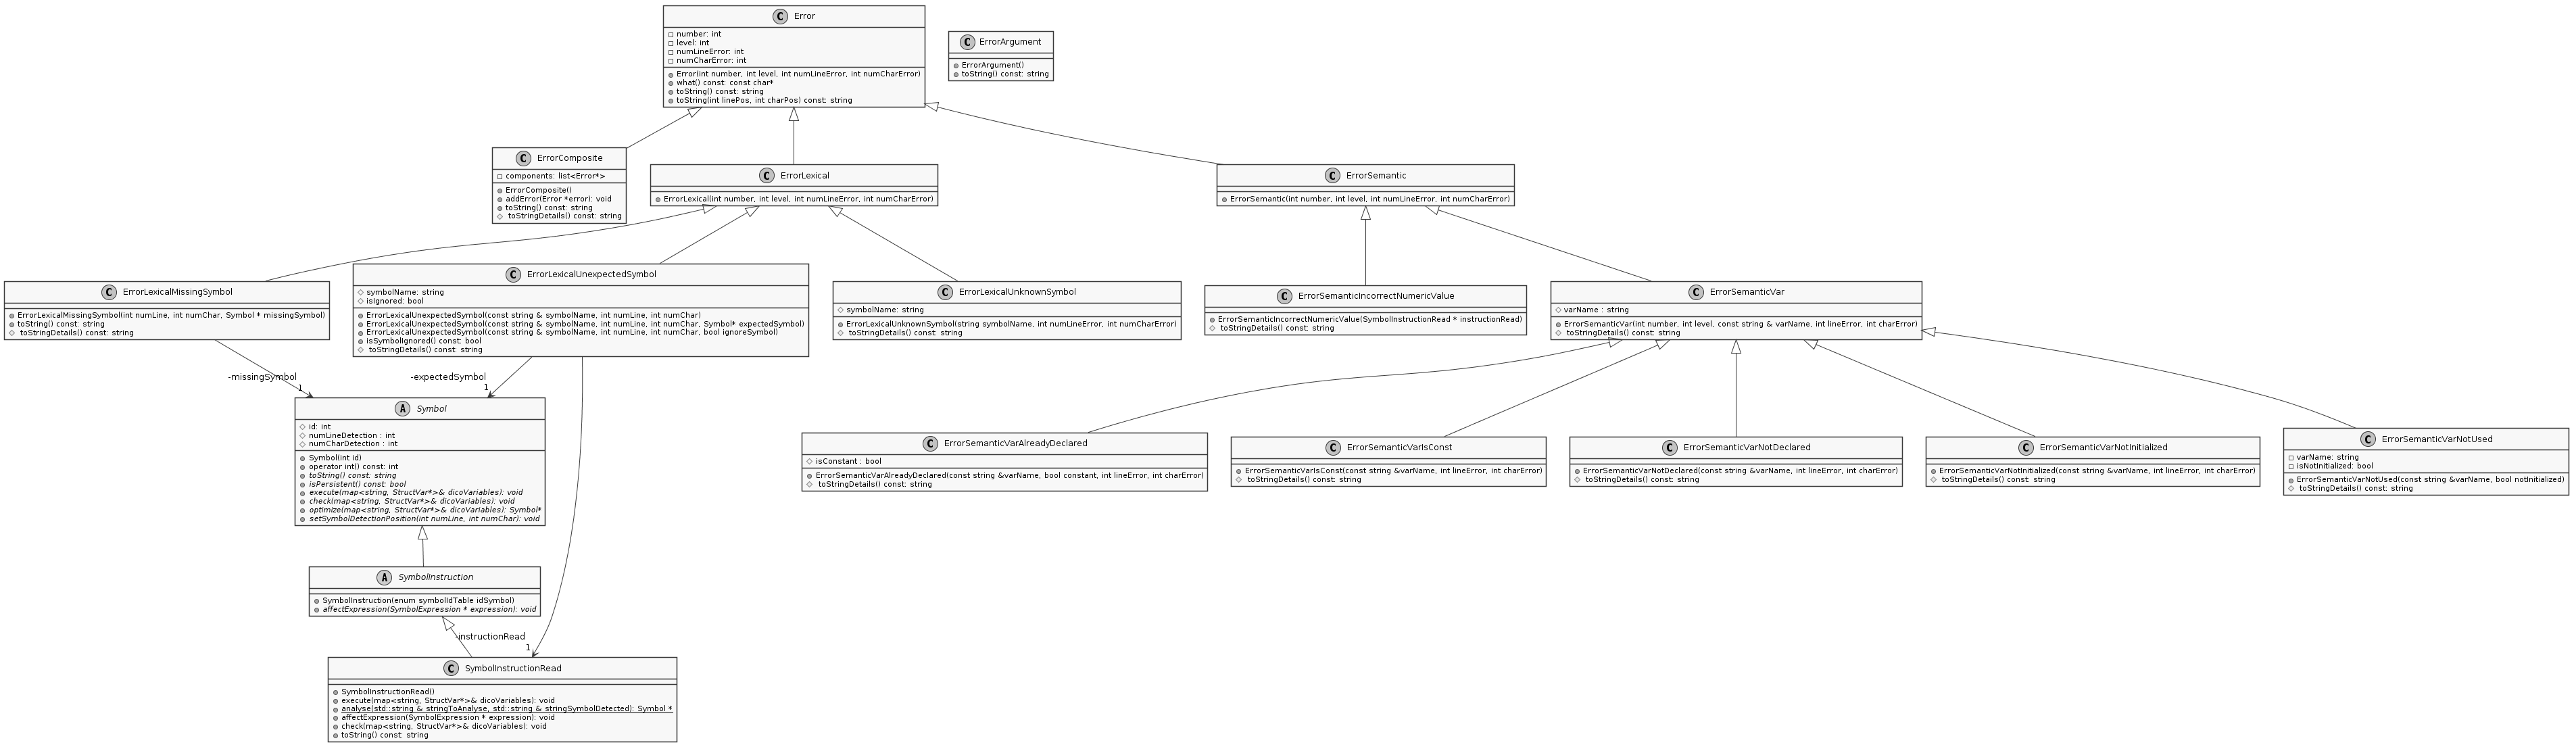
\includegraphics[width=1.0\textwidth,keepaspectratio]{../diagrams-simplified/class/exceptions/lutin-compiler-class-diagram-exceptions-uml.png}
		}	
		\caption{Diagramme de classe des exceptions (erreurs)}
		\label{fig:erreur-structure}
	\end{figure}		
	
	\section{Structures de données complètes}
	\label{sec:full-structure}
	
	\begin{figure}[H]
		\centerline{
			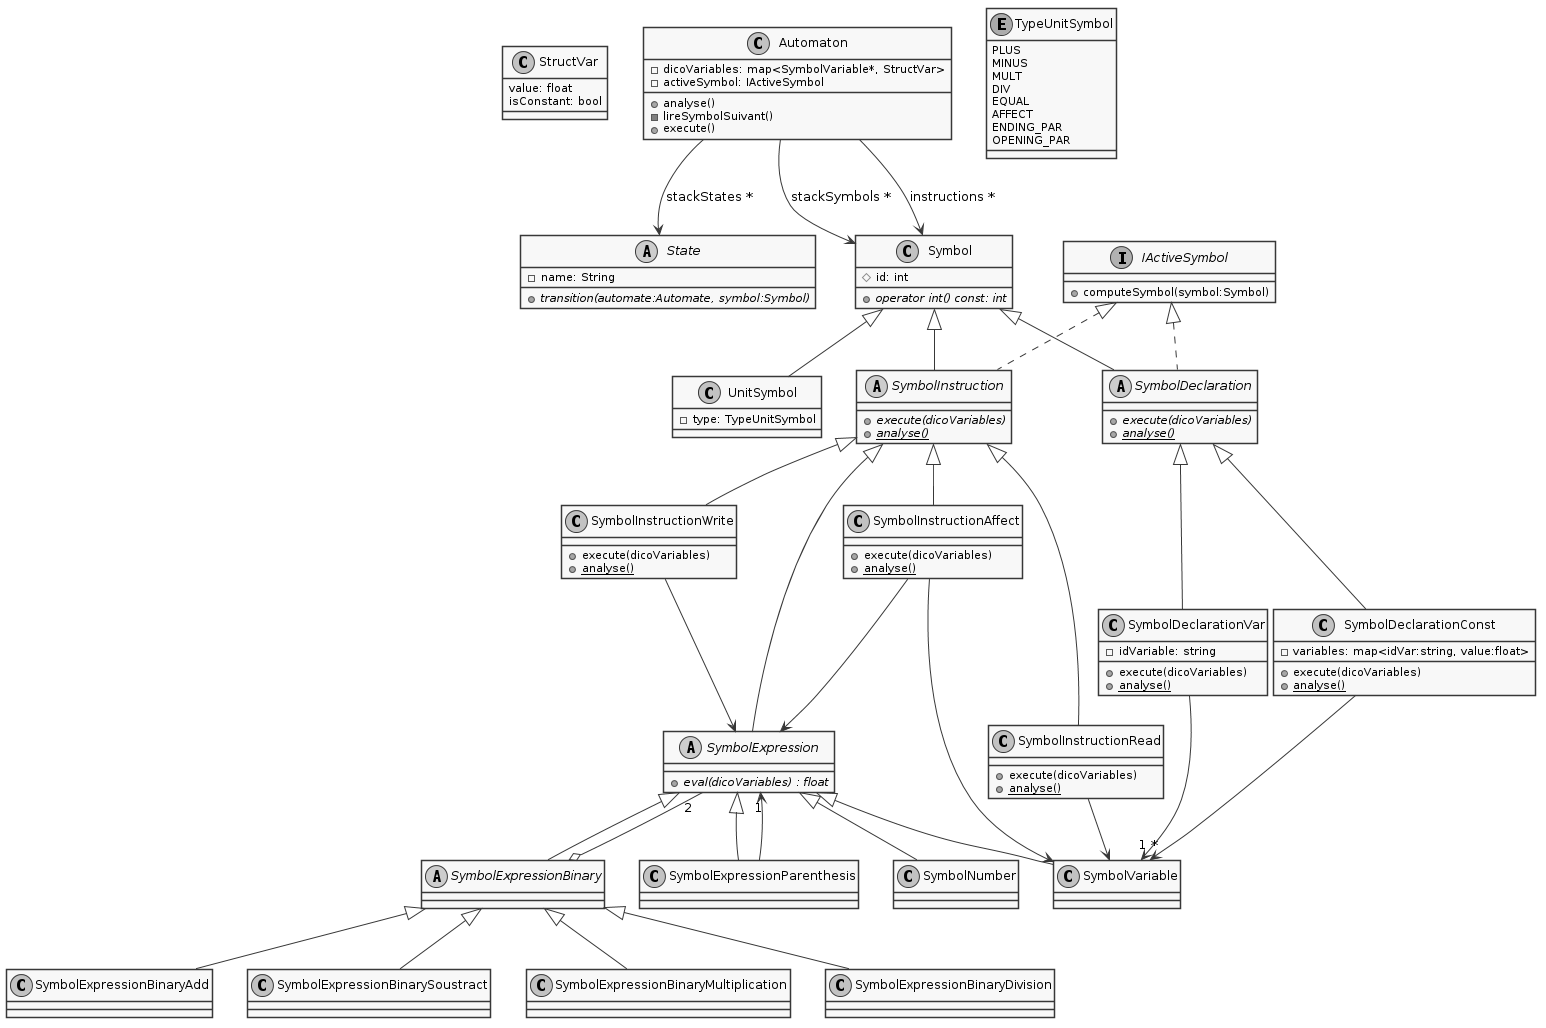
\includegraphics[width=1.15\textwidth,keepaspectratio]{../diagrams/class/lutin-compiler-class-diagram-uml.png}
		}	
		\label{fig:full-structure}
		\caption{Diagramme de classes des structures de données}
	\end{figure}

	\clearpage
	\KOMAoptions{paper=A4,pagesize}
	\recalctypearea
}

%%% End document
\end{document}
